\subsection{Arkitektur}

\begin{figure}[h!]
 \centering
 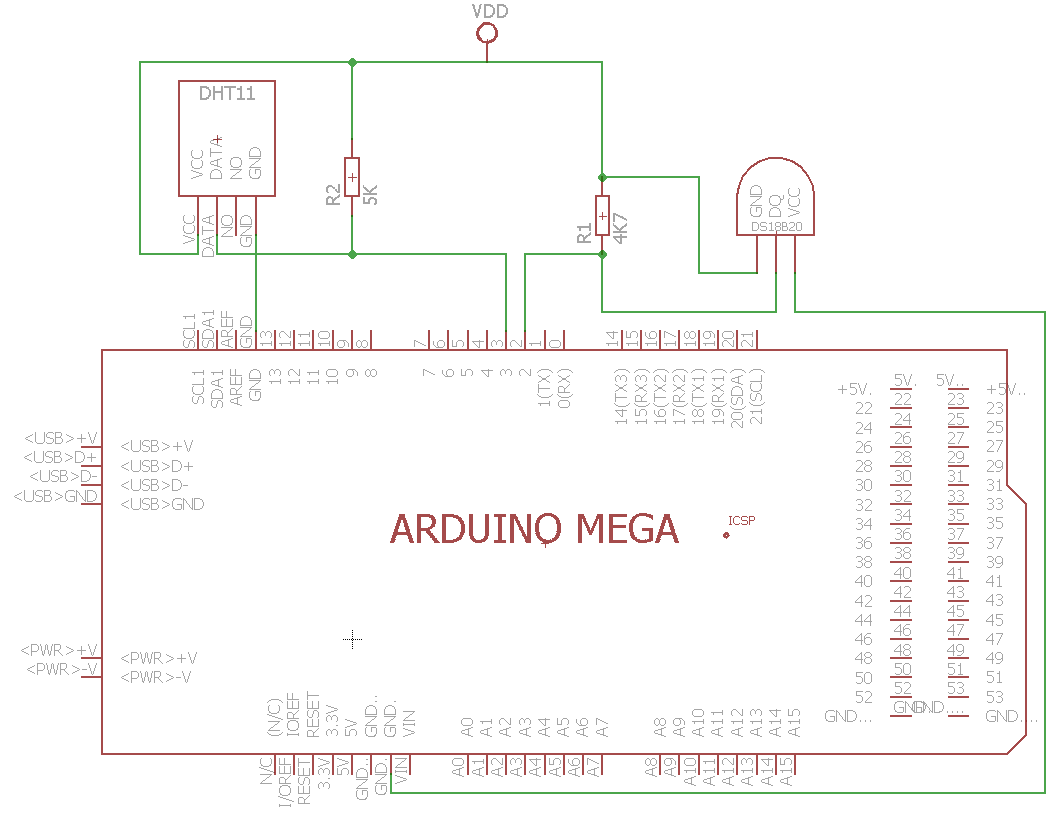
\includegraphics[width=1\textwidth]{figures/phase1_schematic.png}
 \caption{Skematik over mikroprocessor og sensorer.}
 \label{p1_skema}
\end{figure}

Ovenover er vist figur \ref{p1_skema}, som giver et overblik over skemaet af det elektroniske kredsløb brugt til produktet.
Begge sensorer fungerer gennem 1-Wire og deres datalinie er derfor direkte forbundet til mikroprocessoren, og strømtilførslen gennem en modstand.

Til DS18B20 er der valgt at gå væk fra PPM(Parasite Power Mode), hvilket er sensorens måde at modtage strøm gennem datalinien. Denne beslutning blev taget, da det blev valgt bruge sensorens egen temperatur konversion, hvilket ville bruge mere strøm end PPM kan tilføre.
